\chapter{结果与分析}
本次实验共运行了 9 个样例,航行体入射角度分别为 $90 ^\circ$ 垂直入射以及 $60 ^\circ$ 和$45 ^\circ$入射。所有样例的均运行 2 秒,并保留了各运行时段的动力学状态。

\section{稳定的波浪场结果}
在进行完网格划分,边界条件设计,引入动量源项消波法之后,通过合适的数值方法,成功模拟了稳定的波浪场结果。下面为波浪传播某时刻的密度图,压强分布图和速度分布图。

\begin{figure}[!htp]
  \centering
  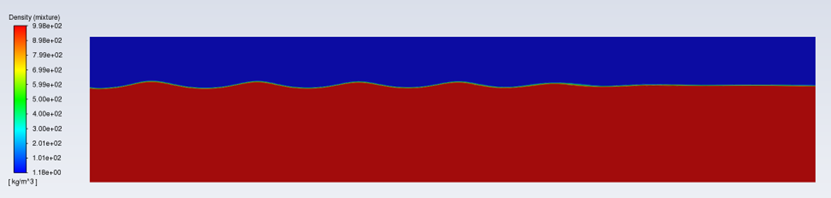
\includegraphics[]{fig/wave_density.png}
  \caption{波浪场密度($\rho$)图}
\end{figure}

波浪场压强分布如图\ref{fig:wave_pressure}所示,可以看到,空气和水体之间的压力区分明显,液体区域随深度增加压强逐渐升高。
\begin{figure}[!htp]
  \centering
  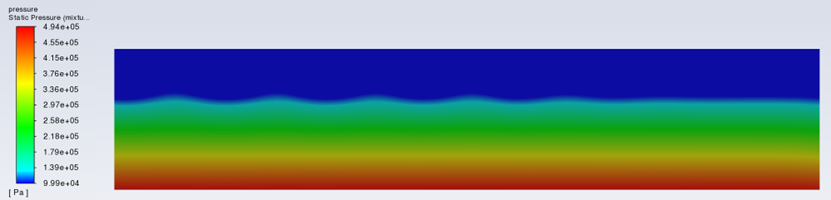
\includegraphics[]{fig/wave_pressure.png}
  \caption{波浪场压强($p$)分布图}
  \label{fig:wave_pressure}
\end{figure}

波浪场速度分布图如图\ref{fig:wave_u},\ref{fig:wave_v}所示,在工作区呈现典型的波浪场速度分布特征,在消波区存在一定的$u$分布,也符合动量源项消波法的结果。
\begin{figure}[!htp]
  \centering
  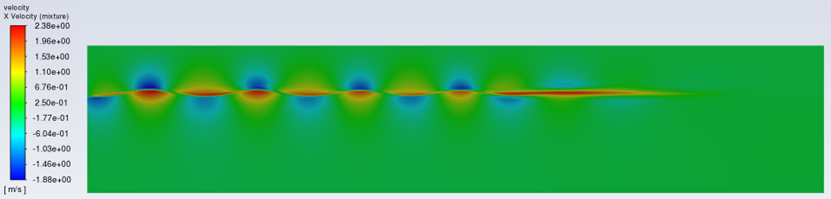
\includegraphics[]{fig/wave_u.png}
  \caption{波浪场$x$方向速度($u$)分布图}
  \label{fig:wave_u}
\end{figure}
\begin{figure}[!htp]
  \centering
  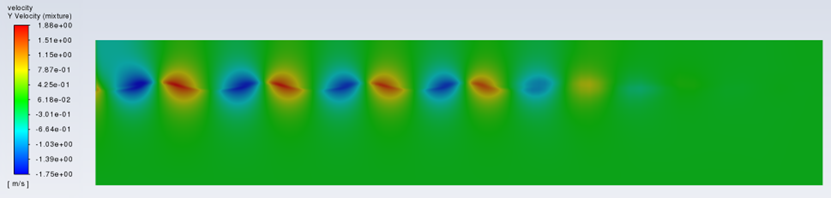
\includegraphics[]{fig/wave_v.png}
  \caption{波浪场$y$方向速度($v$)分布图}
  \label{fig:wave_v}
\end{figure}

\section{不同入水阶段的密度分布}
在考虑并应用 VOF 捕捉方法和重叠网格技术后,可以顺利地进行入水数值模拟实验。数值模拟实验共进行 $t_{\max} = 2s$。以下是入射倾角为 $45^\circ$ 时,运行 $0s$、$0.5$、$0.7s$、$0.9s$、$2.0s$ 的局部密度图。

\begin{figure}[!htp]
  \centering
  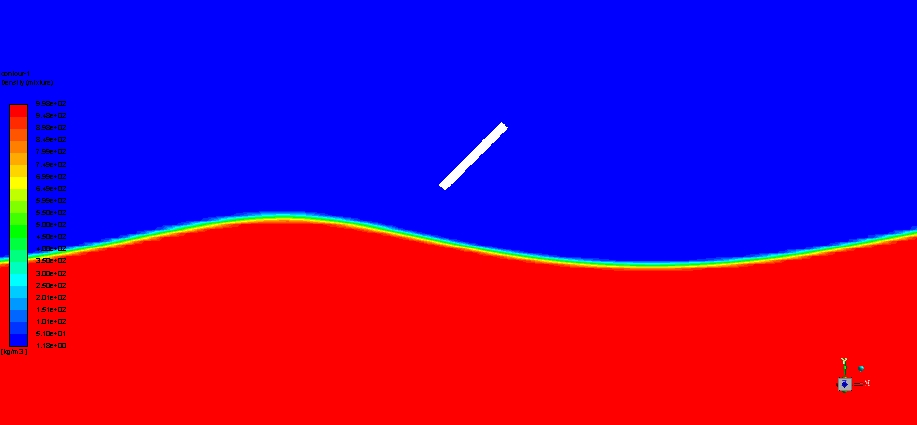
\includegraphics[width=0.5\textwidth]{fig/WaterEntry-AOA45-1-0.jpg}
  \caption{$t=0s$时局部密度图} 
\end{figure}

\begin{figure}[!htp]
  \centering
  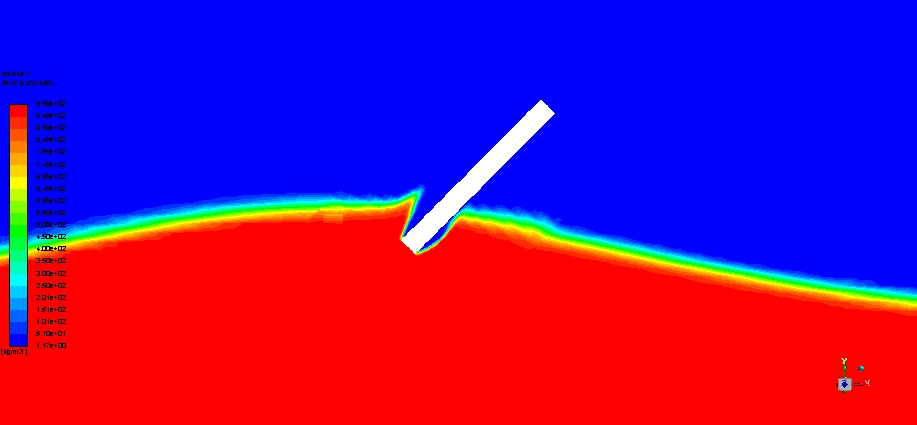
\includegraphics[width=0.5\textwidth]{fig/WaterEntry-AOA45-1-0_5.jpg}
  \caption{$t=0.5s$时局部密度图}
\end{figure}

\begin{figure}[!htp]
  \centering
  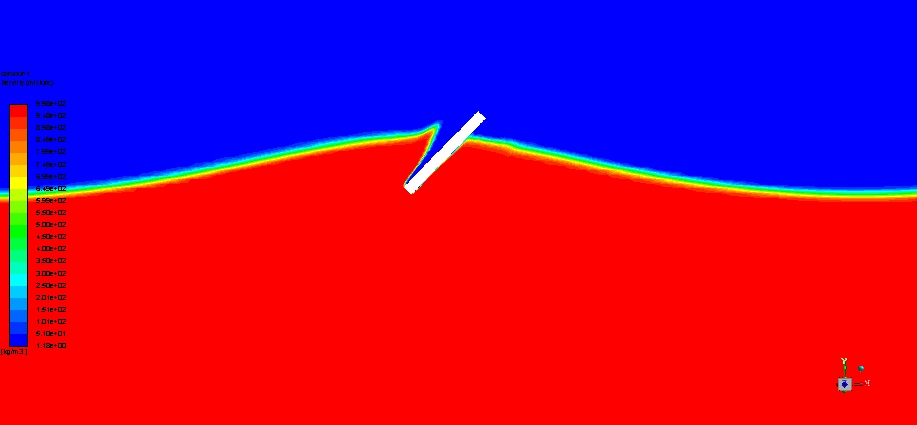
\includegraphics[width=0.5\textwidth]{fig/WaterEntry-AOA45-1-0_7.jpg}
  \caption*{$t=0.7s$时局部密度图} 
\end{figure}

\begin{figure}[!htp]
  \centering
  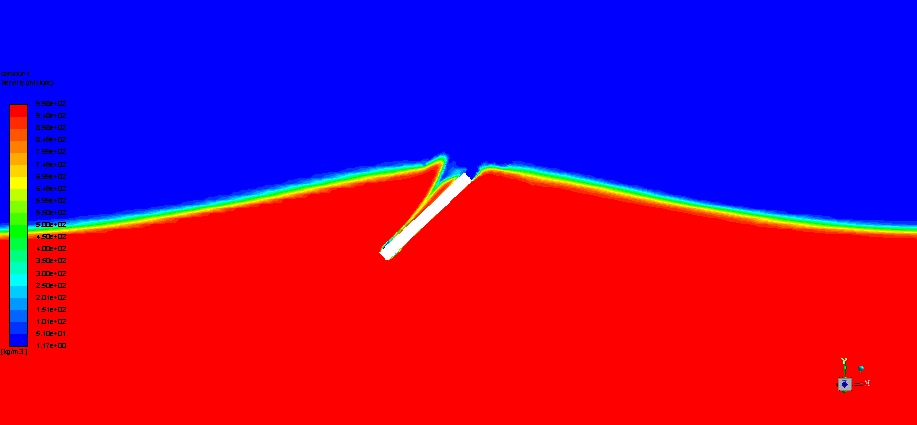
\includegraphics[width=0.5\textwidth]{fig/WaterEntry-AOA45-1-0_9.jpg}
  \caption{$t=0.9s$时局部密度图} 
\end{figure}

\begin{figure}[!htp]
  \centering
  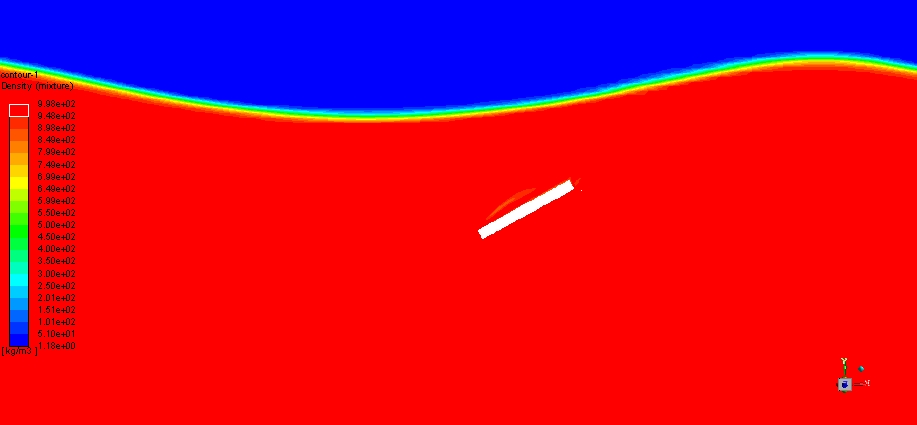
\includegraphics[width=0.5\textwidth]{fig/WaterEntry-AOA45-1-2_000000.jpg}
  \caption{$t=2.0s$时局部密度图} 
\end{figure}

可以看到入水过程发生了显著的空泡现象。